\vspace{1em}
{\bf Horus} is an RDF browser that displays RDF information using a nested box layout. The browser provides a simple navigation paradigm for selecting RDF resources and allows users to switch between different lenses for rendering the resources. Horus supports Fresnel lenses and formats, which can be associated together using Fresnel groups. Groups can refer to external CSS style sheets which are used to define fonts, colors and borders. Horus supports basic selectors, but does not offer SPARQL and FSL as selector languages. Horus is implemented using PHP and is backed by a MySQL database. Applying a lens to an RDF resource results in an intermediate tree, which is formatted afterwards using the formats that are associated to the group of the selected lens. The ordered and formatted intermediate tree is then serialized into XHTML.  

\begin{figure}
\begin{tabular}{cc}
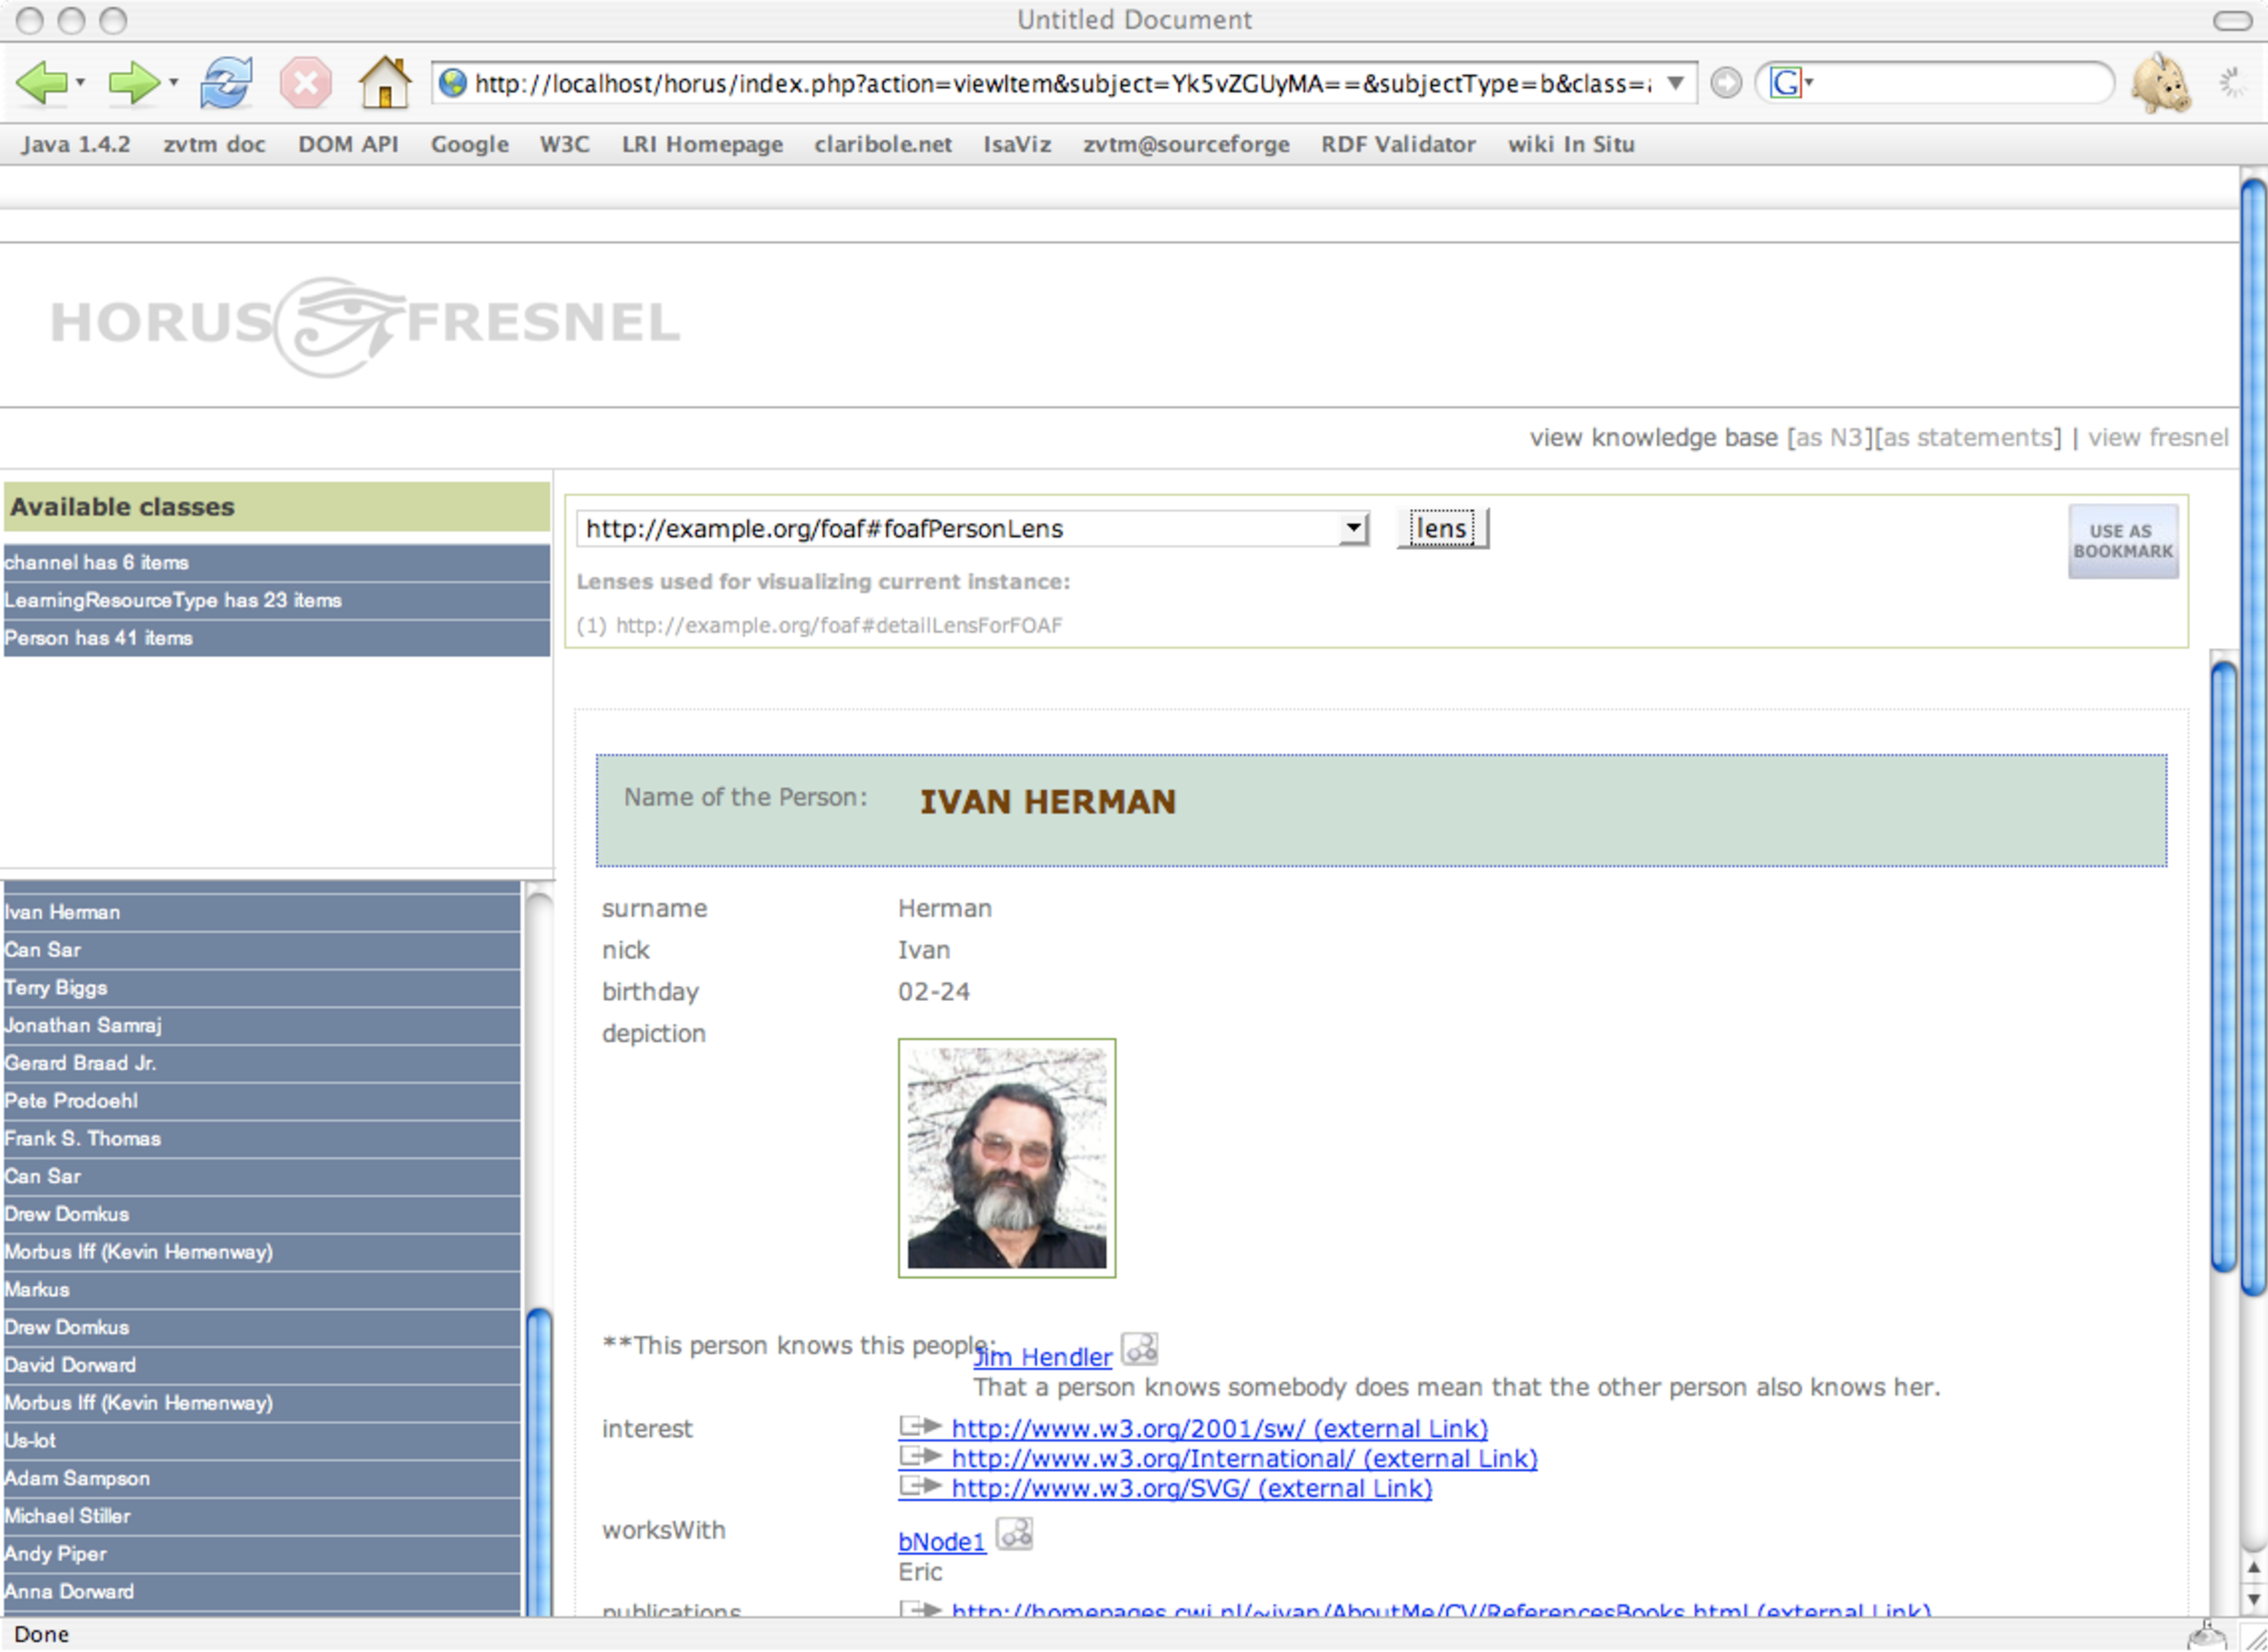
\includegraphics[width=6cm]{horus1.pdf} \hspace{0.02cm} &
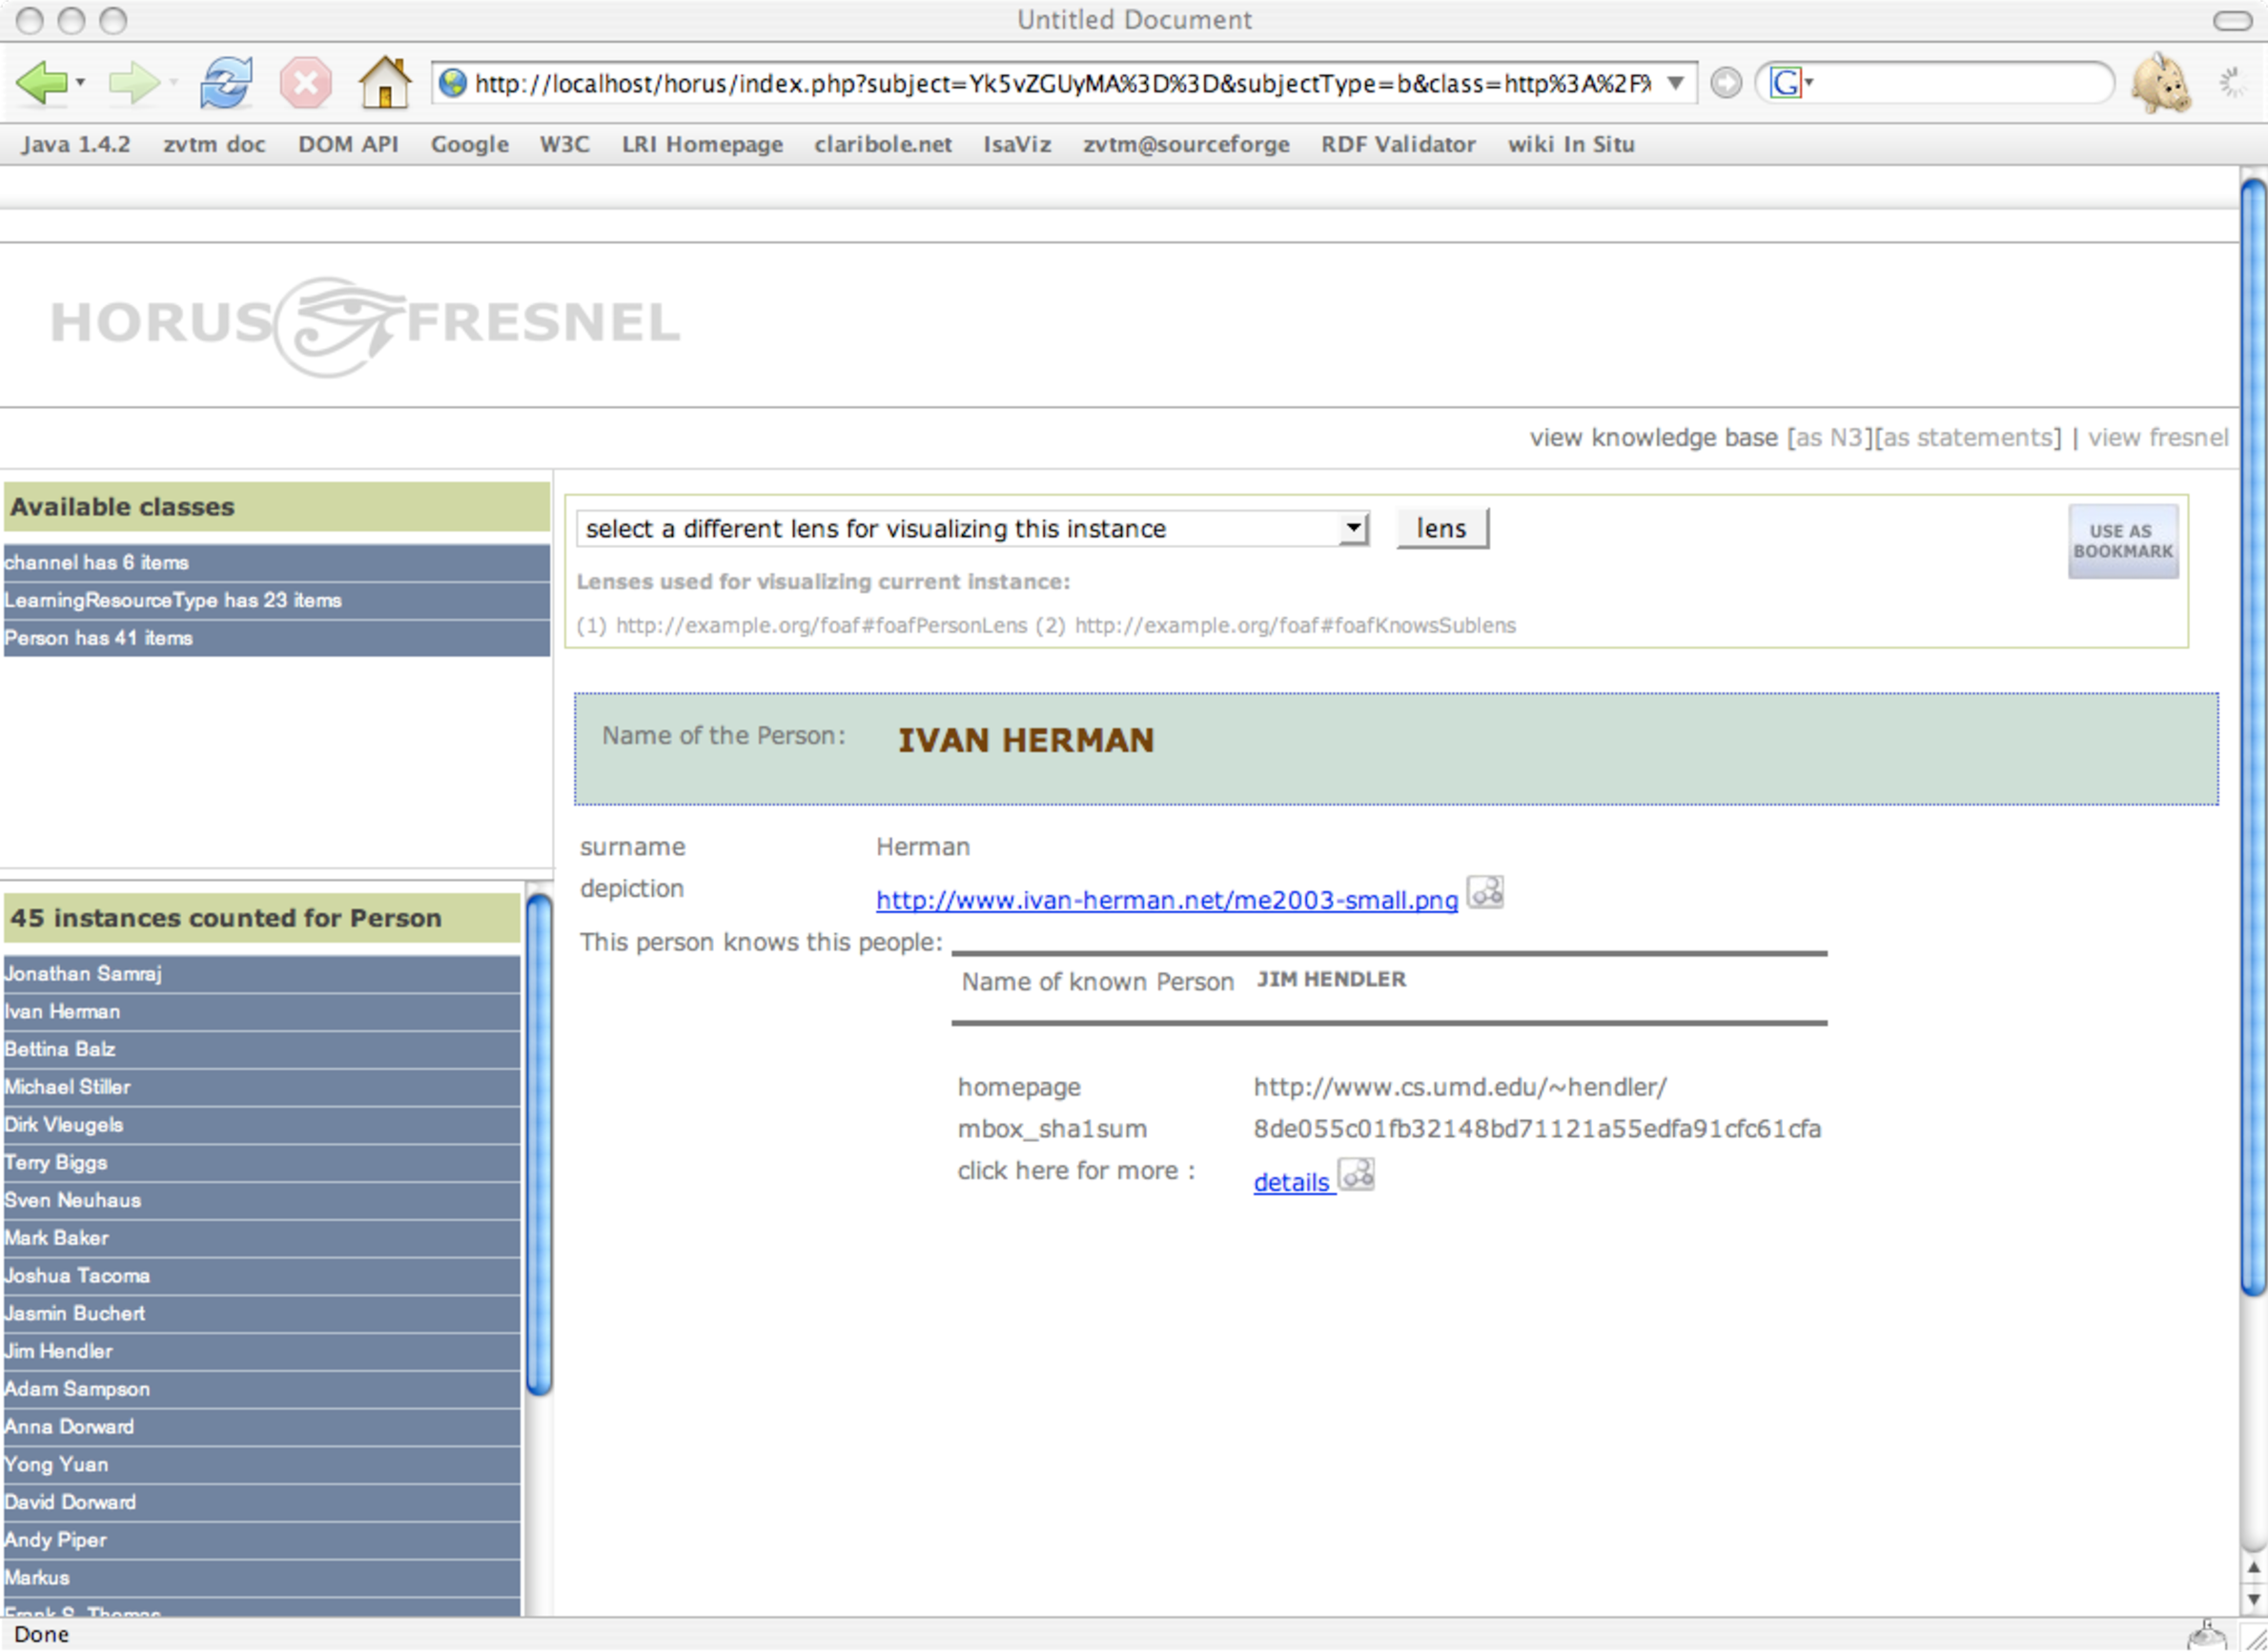
\includegraphics[width=6cm]{horus2.pdf} \\
\end{tabular}
\vspace{-1em}
\caption{Two different views on the same person in Horus: detailed view (left), friends view (right)}
\label{horusFig1}
\vspace{-1.1em}
\end{figure}

Figure \ref{horusFig1} shows two different views on the same person in Horus. The view on the left uses a lens that displays many details about persons. The sentence "{\em This person knows the following people}" is a custom label for property \rdf{foaf:knows}. The disclaimer "{\em That a person knows somebody does\ldots}" is static content added using property \rdf{fresnel:contentLast}. Some of the links are formatted as external links (\rdf{fresnel:value} formatting instruction set to \rdf{fresnel:externalLink}), while others refer to RDF resources in the knowledge base, and thus have a different rendering.

%\begin{figure}
%\begin{center}
%\begin{tabular}{c}
%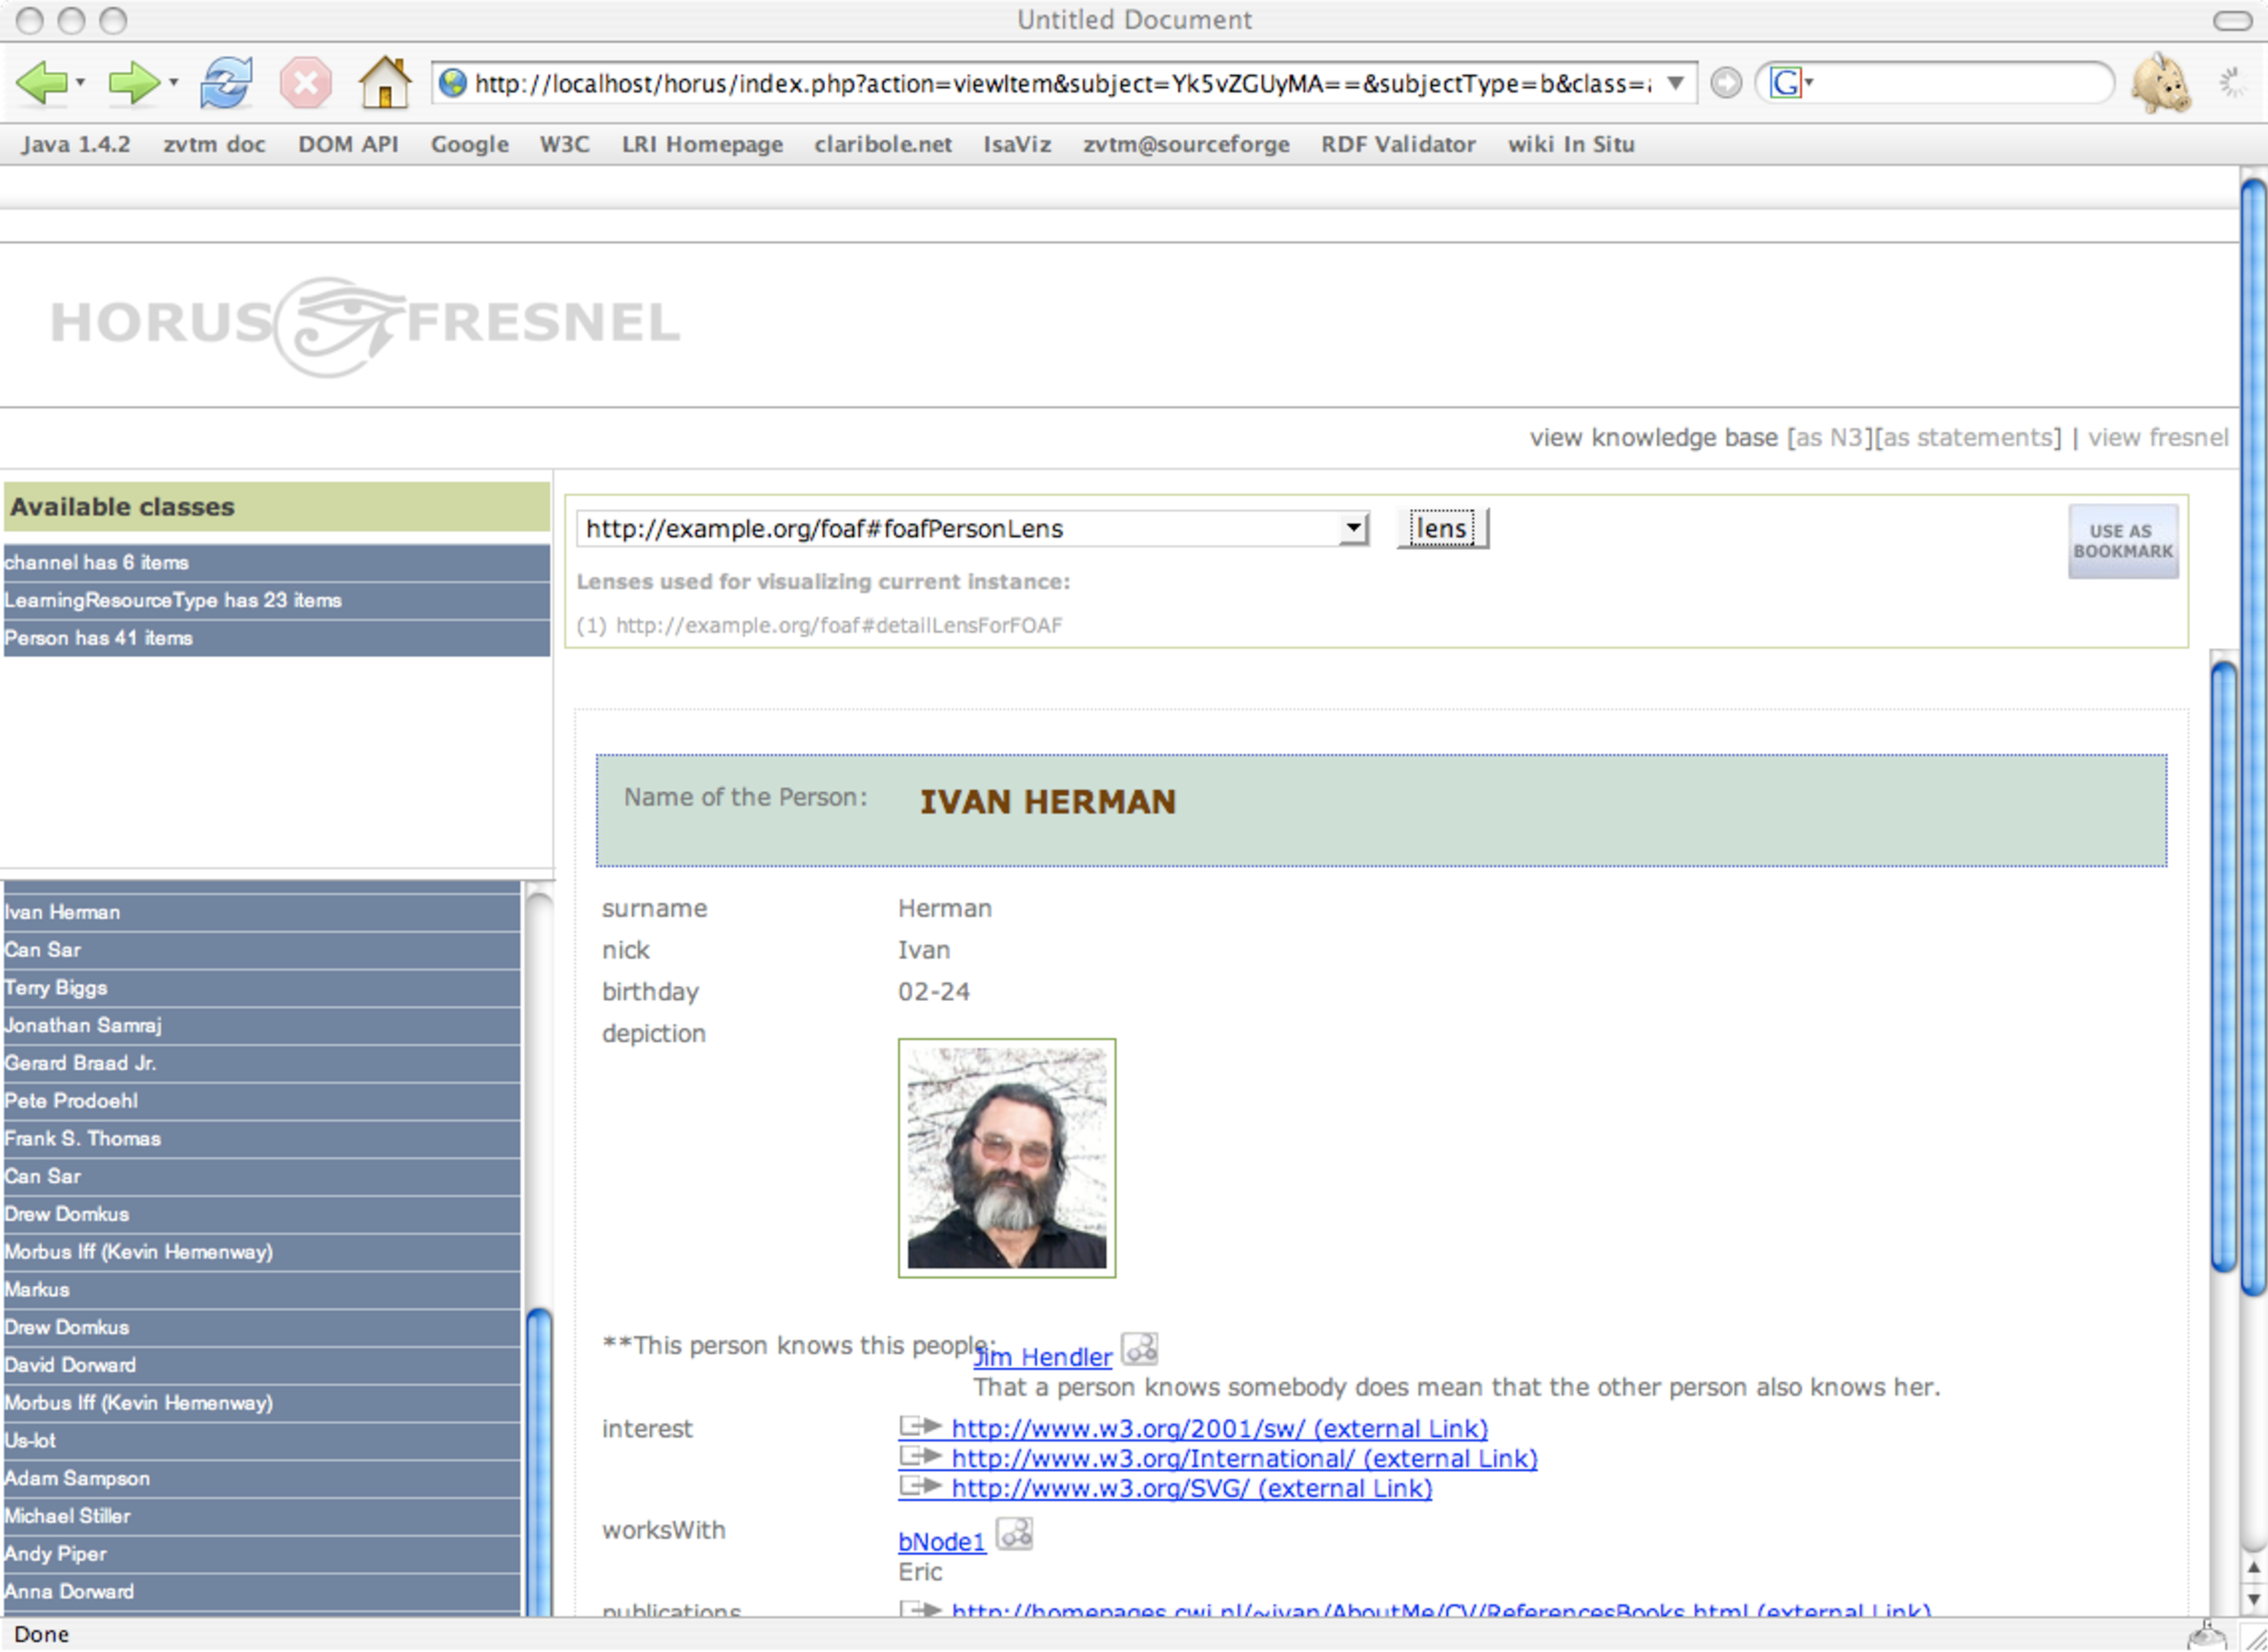
\includegraphics[width=10cm]{horus1.pdf} \\
%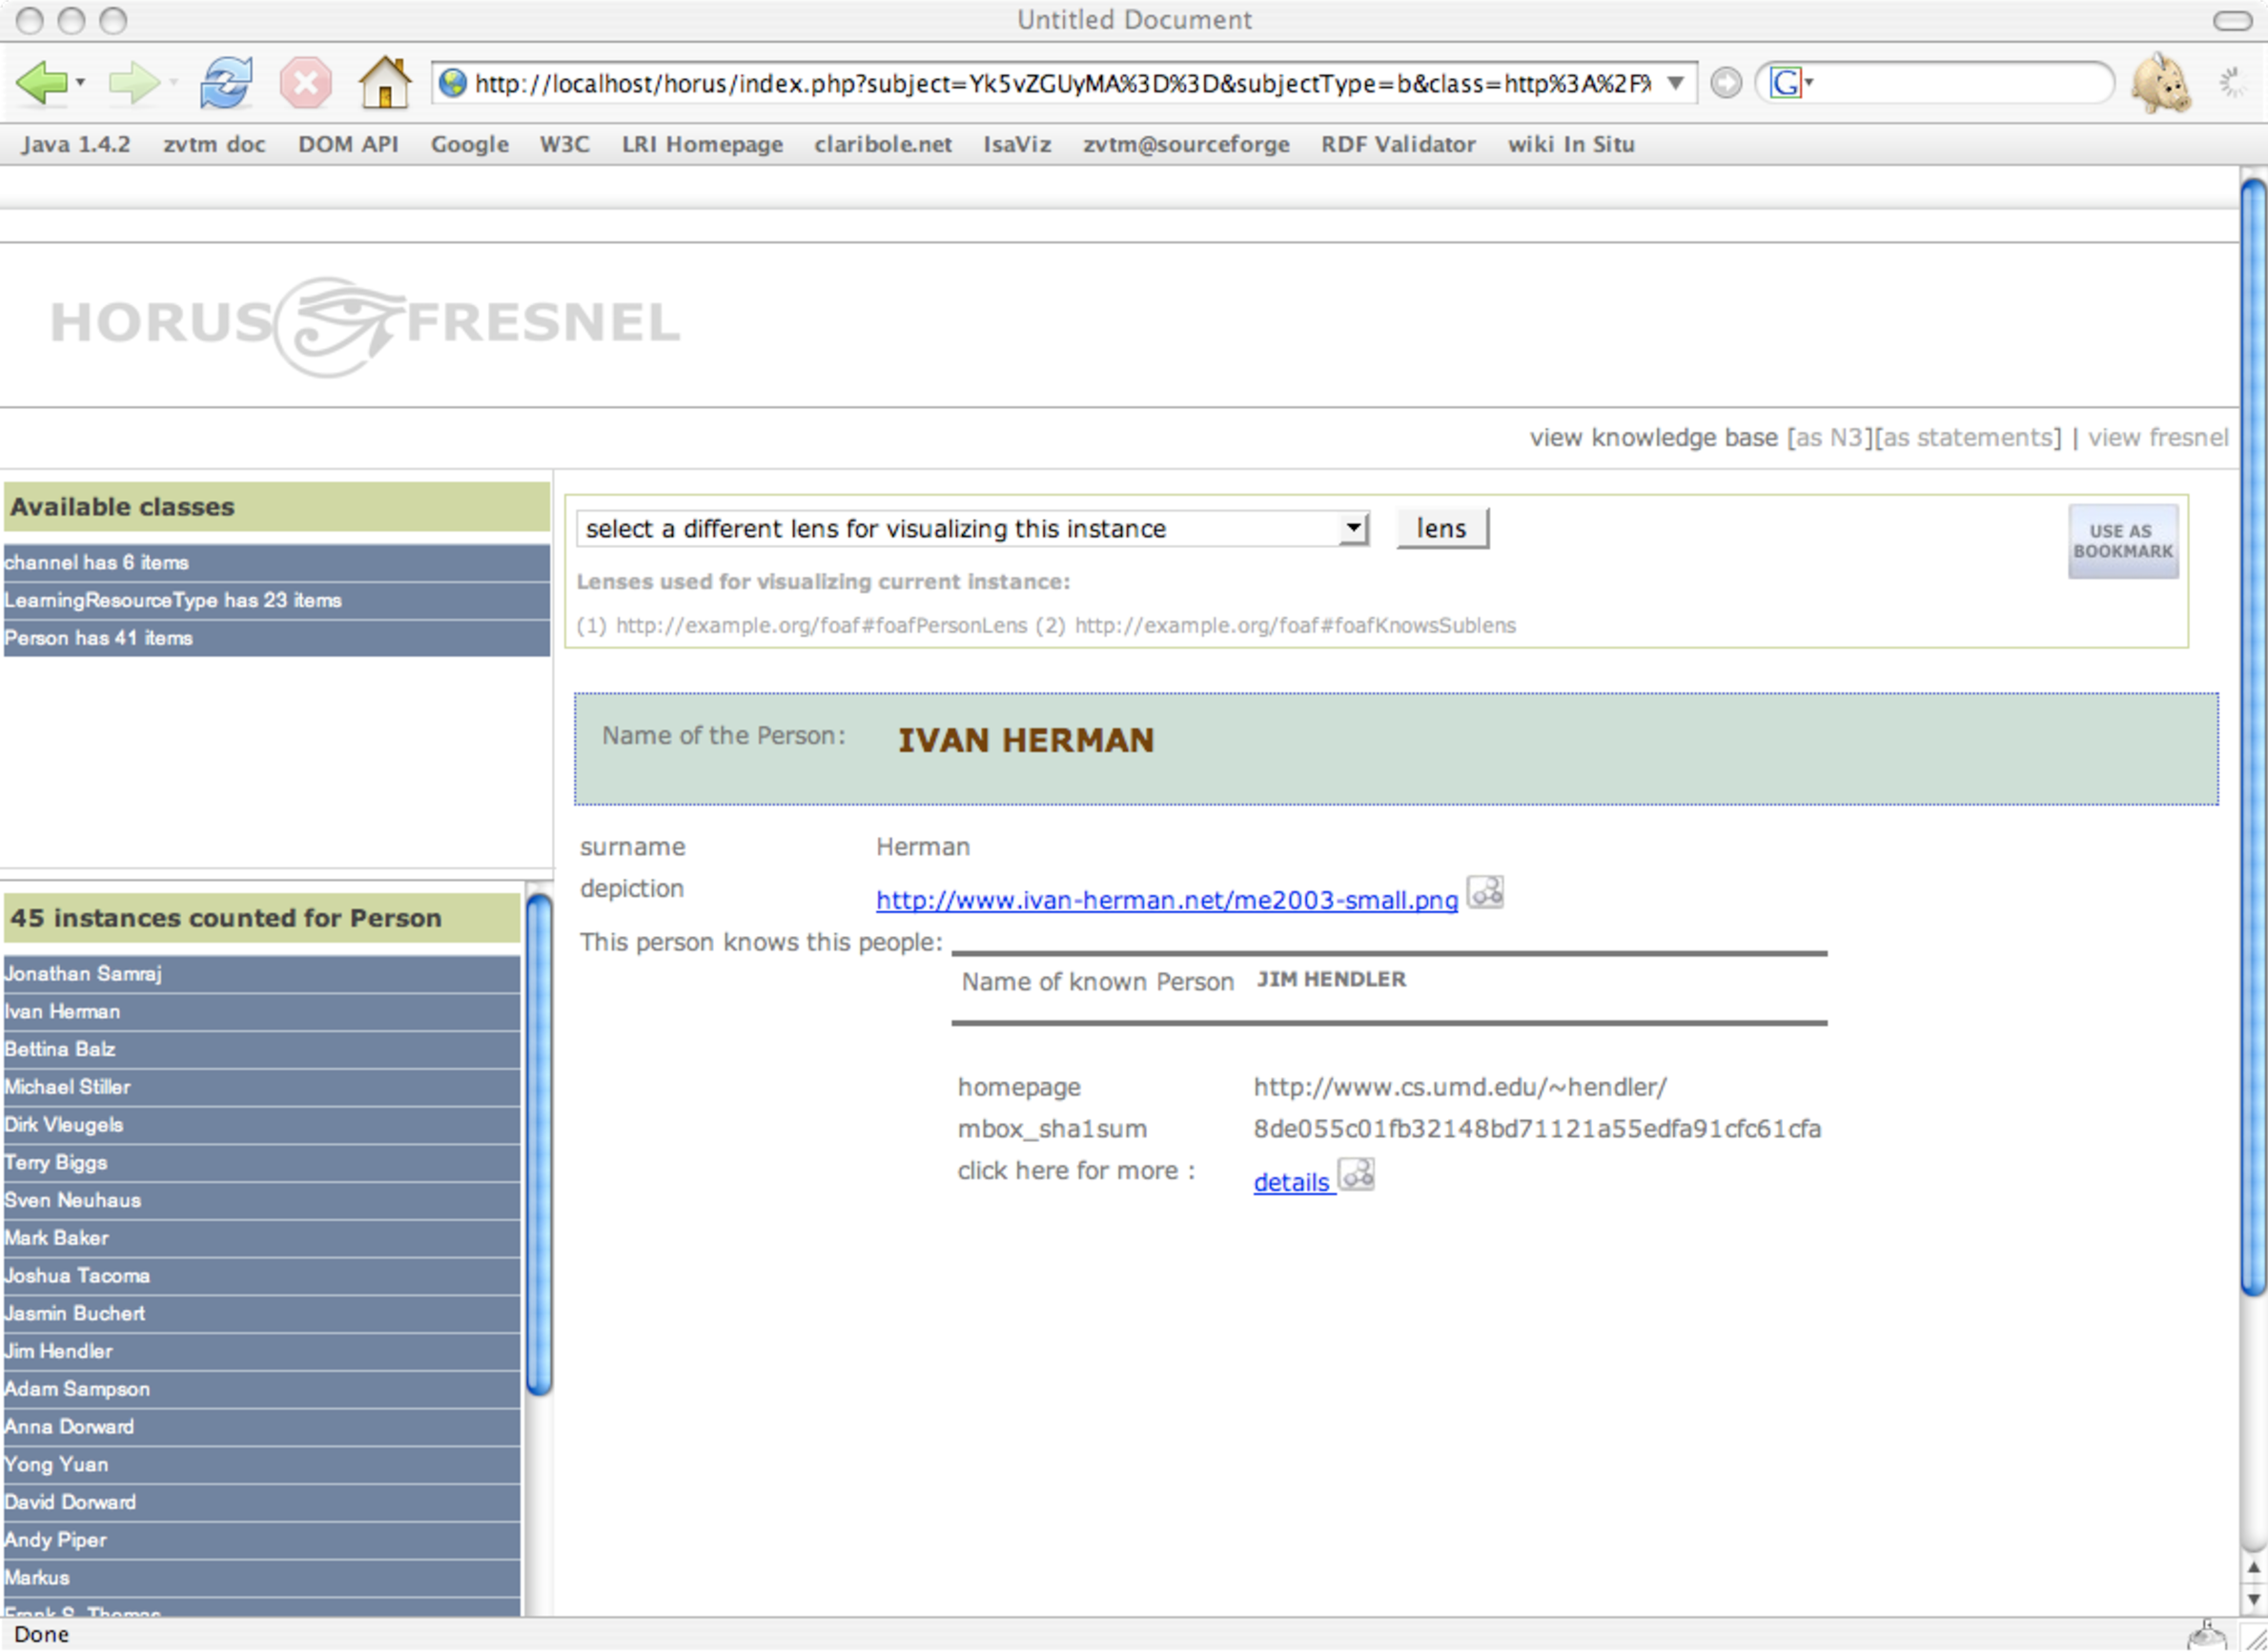
\includegraphics[width=10cm]{horus2.pdf}
%\end{tabular}
%\end{center}
%\caption{Two different views on the same person in Horus: detailed view (left), friends view (right)}
%\label{horusFig1}
%\end{figure}


On the right side of Figure \ref{horusFig1}, the same person is shown using a different lens. This lens displays less details about the person itself, but refers to a second lens (used as a sublens) for displaying details about other persons known by this person. As the sublens belongs to a different group, another CSS class is used to style the names of the person's friends.
